\chapter{Detailed design}

In this chapter, every single class is described in terms of public interface
and functionality. Because of the fairly dynamic character of this project --
new ideas come and go -- this chapter will not be finished until the end of the
project and will probably change regularly.

\section{Files and directories}

All source code will be in the directory \texttt{src/}. All classes are in the
package \texttt{amber} or in a subpackage thereof. The Psyclone specification
file \texttt{psySpec.xml} is found in \texttt{data/}. External libraries that
are redistributed with \Amber\ are in \texttt{lib/}. The source of this
document, the traineeship report and the website are located in
\texttt{documentation/}.

The application is built using Apache
Ant\footnote{\url{http://ant.apache.org/}} and it can be imported into
Eclipse\footnote{\url{http://www.eclipse.org/}}. It requires Java SDK version
1.5 or greater.

%%%%%%%%%%%%%%%%%%%%%%%%%%%%%%%%%%%%%%%%%%%%%%%%%%%%%%%%%%%%%%%%%%%%%%%%%%%%%%%%
\section{Classes in the amber package}

The classes in the main package are launchers for the three different modules
and abstract classes for the main objects of these modules. Basically it works
like this; if the Crawler class is started it creates a CrawlerObject and
starts it.

\classname{Crawler}

\begin{classmetadata}
\end{classmetadata}

\begin{classinterface}
\end{classinterface}



\classname{CrawlerObject}

\begin{classmetadata}
\end{classmetadata}

\begin{classinterface}
\end{classinterface}



\classname{ShowOff}

\begin{classmetadata}
\end{classmetadata}

\begin{classinterface}
\end{classinterface}



\classname{ShowOffObject}

\begin{classmetadata}
\end{classmetadata}

\begin{classinterface}
  \method{\void}{start}{}
    {Starts the ShowOff module.}
  \method{\void}{stop}{}
    {Stops the ShowOff module.}
  \method{\void}{setStoryQueue}{Queue$\langle$Story$\rangle$ q}
    {Sets the queue of incoming stories. ShowOff will handle communication with
    the Psyclone whiteboard and puts stories in the queue.}
\end{classinterface}



\classname{Sieve}

\begin{classmetadata}
\end{classmetadata}

\begin{classinterface}
\end{classinterface}



\classname{SieveObject}

\begin{classmetadata}
\end{classmetadata}

\begin{classinterface}
\end{classinterface}



%%%%%%%%%%%%%%%%%%%%%%%%%%%%%%%%%%%%%%%%%%%%%%%%%%%%%%%%%%%%%%%%%%%%%%%%%%%%%%%%
\section{Classes in the amber.common package}

\classname{AirBrush}

\begin{classmetadata}
\end{classmetadata}

\begin{classinterface}
\end{classinterface}



\classname{Configuration}

\begin{classmetadata}
\end{classmetadata}

\begin{classinterface}
\end{classinterface}



\classname{Object}

\begin{classmetadata}
\end{classmetadata}

\begin{classinterface}
\end{classinterface}



\classname{Story}

\begin{classmetadata}
  \function{Storage of Story data.}
  \data{Story has a Map$\langle$String, Object$\rangle$ field where it stores
    all data. It also holds a value with the number of analyses left until it
    is considered enough to be visualized. Instead of thrown back on the
    whiteboard with raw stories, it should then go the the processed stories.}
\end{classmetadata}

\begin{classinterface}
  \method{\void}{setAuthor}{String}{Sets the author of the story.}
  \method{String}{getAuthor}{}{Gets the author of the story.}
  \method{\void}{setCreationTime}{Date}{Set the creation time of the story}
  \method{Date}{getCreationTime}{}{Get the creation time of the story.}
  \method{\void}{setContent}{String}{Set the content of the story.}
  \method{String}{getContent}{}{Get the content of the story.}
  \method{\void}{setValue}{String k, Object v}
    {Sets an arbitrary object v under keyword k.}
  \method{Object}{getValue}{String k}
    {Gets the object v stored under keyword k.}
  \method{Boolean}{lockForAnalysis}{}
    {Request a lock on the story for analysis. Returns true when given, assumes
      niceness of the analysis modules.}
  \method{\void}{unlock}{}
    {Removes the lock. Again, assumes niceness of the analysis modules.}
  \method{Boolean}{isAnalysisDone}{}
    {Returns true when the story finds it is analysed enough and doesn't need
      another run.}
\end{classinterface}



%%%%%%%%%%%%%%%%%%%%%%%%%%%%%%%%%%%%%%%%%%%%%%%%%%%%%%%%%%%%%%%%%%%%%%%%%%%%%%%%
\section{Classes in the amber.crawler package}

\classname{Configuration}

\begin{classmetadata}
\end{classmetadata}

\begin{classinterface}
\end{classinterface}



\classname{RSS}

\begin{classmetadata}
\end{classmetadata}

\begin{classinterface}
\end{classinterface}



\begin{figure}
  \centering
  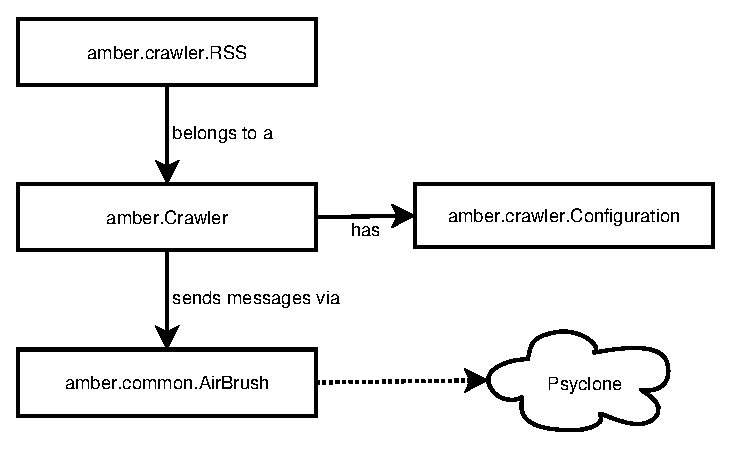
\includegraphics{image/crawler}
  \caption{
    Diagram of the design of the Crawler, the names are Java classnames
  }
\end{figure}


%%%%%%%%%%%%%%%%%%%%%%%%%%%%%%%%%%%%%%%%%%%%%%%%%%%%%%%%%%%%%%%%%%%%%%%%%%%%%%%%
\section{Classes in the amber.sieve package}

\classname{Configuration}

\begin{classmetadata}
\end{classmetadata}

\begin{classinterface}
\end{classinterface}



\classname{KeywordSpotter}

\begin{classmetadata}
\end{classmetadata}

\begin{classinterface}
\end{classinterface}



%%%%%%%%%%%%%%%%%%%%%%%%%%%%%%%%%%%%%%%%%%%%%%%%%%%%%%%%%%%%%%%%%%%%%%%%%%%%%%%%
\section{Classes in the amber.showoff package}

\classname{Configuration}

\begin{classmetadata}
  \ancestor{amber.common.Configuration}
  \function{Store configuration}
\end{classmetadata}

\begin{classinterface}
  \method{void}{setValue}{String key}
    {Sets the value of key in the configuration.}
\end{classinterface}



\classname{EarthView}

\begin{classmetadata}
  \extends{java.awt.Canvas}
  \implements{Runnable}
\end{classmetadata}

\begin{classinterface}
  \init{EarthView}{}
    {Initializes the earthview display. It is a child of Canvas and can as such
    be used inside any application. Before starting the Earthview, first couple
    a Particle collection to it using setParticleCollection.}
  \method{\void}{setParticleCollection}{pc: Collection$\langle$Particle$\rangle$}
    {Sets the collection of particles to be displayed in the view.}
  \method{\void}{run}{}
    {Runs the thread (for Runnable).}
  \method{\void}{start}{}
    {Starts the thread, lets EarthView draw stuff.}
\end{classinterface}



\classname{FullScreen}

\begin{classmetadata}
  \ancestor{amber.ShowOffObject}
  % \function{}
\end{classmetadata}

\begin{classinterface}
  \init{FullScreen}{}
    {Initializes something.}
  \method{\void}{start}{}
    {Start the visualization.}
\end{classinterface}



\classname{Particle}

\begin{classmetadata}
  \function{Storage of particle data.}
  \data{An object of this class has information about its location and
    velocity, and it knows from which story it originates.}
\end{classmetadata}

\begin{classinterface}
  \init{Particle}{Story s}
    {Initializes a particle for Story s.}
  \method{\void}{launch}{}
    {Launches the particle, all parameters must be set, they cannot be changed
      afterwards.}
  \method{\void}{boost}{double}
    {Boost the particle in the direction it is heading. This can happen when
      for instance the Story gets replies or comments; boosting keeps the
      particle around longer.}
  \method{double}{getMass}{}
    {Gets the mass of the particle}
  \method{Vector$\langle$double$\rangle$}{getLocation}{}
    {Gets the location}
  \method{Vector$\langle$double$\rangle$}{getVelocity}{}
    {Gets the velocity}
  \method{Vector$\langle$double$\rangle$}{getAcceleration}{}
    {Gets the acceleration}
  \method{\void}{setMass}{double s}
    {Sets the mass of the particle to s}
  \method{\void}{setLocation}{Vector$\langle$double$\rangle$ v}
    {Sets the location to v}
  \method{\void}{setVelocity}{Vector$\langle$double$\rangle$ v}
    {Sets the velocity to v}
  \method{\void}{setAcceleration}{Vector$\langle$double$\rangle$ v}
    {Sets the acceleration to v}
  \method{\void}{setNewValuesAfter}{double t}
    {Calculates and sets new values using the current values after a period of
      time t}
\end{classinterface}



\classname{Applet}

\begin{classmetadata}
  \extends{java.applet.Applet}
\end{classmetadata}

\begin{classinterface}
\end{classinterface}



\begin{figure}
  \centering
  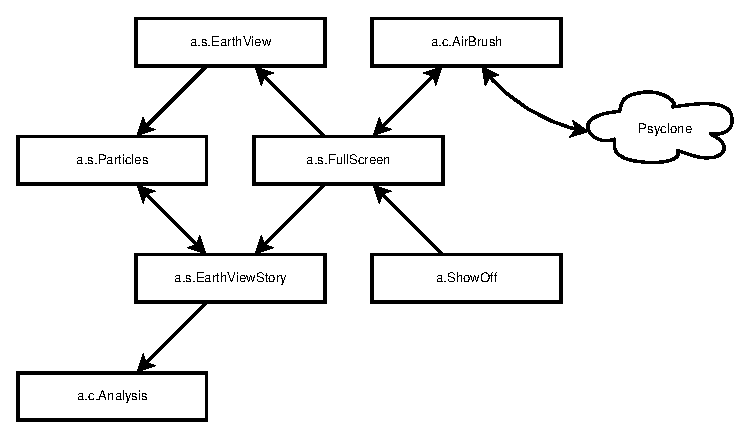
\includegraphics{image/showoff-fullscreen}
  \caption{
    Diagram of the design of the full screen ShowOff module, the names are
    abbreviated Java classnames
  }
\end{figure}


